\chapter{Contexte et concepts}

%another definition


      
%end of other definition

Aujourd'hui, sur internet des entreprises mettent à disposition de leurs utilisateurs un nombre colossal de données comme YouTube, Amazon ou encore Netflix. Ainsi, il est devenu difficile pour l'utilisateur de trouver des informations pertinentes rapidement. Diverses techniques informatiques se sont développées pour contourner ce problème et ce bien avant les géants d'internet que nous connaissons. Dans le cadre de ce mémoire, nous nous intéresseront essentiellement aux systèmes de recommandation.


\vspace{5mm}

En 1967\supercite{MACQUEEN}, James McQueen applique un algorithme K-moyennes (K-means) permettant de construire des portions de populations homogènes selon plusieurs critères définis à l’avance. Actuellement, cette première étape est considérée comme le début de la recommandation personnalisée. En 1979, est crée Grundy\supercite{Grundy}, il s'agit d'une tentative de recommandation automatique appliquée au métier de bibliothécaire. A l'aide d'une interview, le système classe les utilisateurs en "stéréotypes" permettant ainsi de recommander différents livres en fonctions de leurs "stéréotypes". Nous pouvons considérer qu'il s'agit de la première réelle application d'un système de recommandation. 



\section{Généralités}

Un système de recommandation est une forme spécifique de filtrage de l’information qui a pour but de présenter à un utilisateur des éléments qui sont susceptibles de l’intéresser. Ce système fonctionne en se basant sur les préférences et le comportement d'un utilisateur ou d'un groupe d'utilisateur. In fine, un système de recommandation tente donc de prédire si un élément suggéré est  succeptible d'être apprécié par un utilisateur donné. 

\vspace{5mm} 

Aujourd'hui, les systèmes de recommandations sont devenus êxtremements populaires, ils sont utilisés dans de nombreuses webapp et appliqués à de nombreux domaines comme la publicité, la vente de masse ou encore la consommation de contenu.

\vspace{5mm}

Actuellement, le nombre de données collectées par des entreprises comme Google par exemple, augmente de façon exponentielle, en raison de cette croissance l'importance des systèmes de recommandation augmente tout autant. Depuis les années 90, les systèmes de recommadation sont devenus un domaine de recherche autonome et en recherche constante d'évolution\supercite{ieee}.



%l'intérêt des utilisateurs. Ancien travail [10] distingue recommandation
%techniques en suivant quatre classes.

\section{Les différentes approches}

%[http://citeseerx.ist.psu.edu/viewdoc/download?doi=10.1.1.695.6428&rep=rep1&type=pdf]

%[https://interstices.info/les-systemes-de-recommandation-categorisation/]

Il existe une multitude de type de données avec chacunes des spécificités différentes. Pour être le plus efficace possible, il existe différentes implémentations des systèmes de recommandation afin de traiter au mieux les données utilisateurs permettant d'apporter l'information la plus pertinante possible.

\vspace{5mm} 

En me basant sur les travaux d'Elsa NEGRE\supercite{elsaNegre}(Maître de Conférences à l'Université Paris - Dauphine), j'ai pu déterminer l'existance de 3 grands types de systèmes de recommandation : basé sur un filtrage collaboratif, filtré sur le contenu et enfin les systèmes hybrides. Chacun de ses types de systèmes de recommandation permet de s'adapter au mieux en fonction des différents besoins.


\subsection{Le filtrage collaboratif}

Les systèmes basés sur le filtrage collaboratif construisent des recommandations en observant  la similarité entre les préférences d’un utilisateur et celles d’autres utilisateurs. Ce système ne permet pas d'analyser ou d'étudier les éléments à recommander mais à faire des prévisions basées sur les intérêts d'un utilisateur comparé à un ensemble d'utilisateurs ayant un profil similaire. Dans ce système, on suppose que plus le profil d'un utilisateur est proche d'un ensemble/groupe d'utilisateur alors ils auront tendance à aimer les mêmes éléments. 

\vspace{5mm}

\begin{figure}[htp]
  \centering
  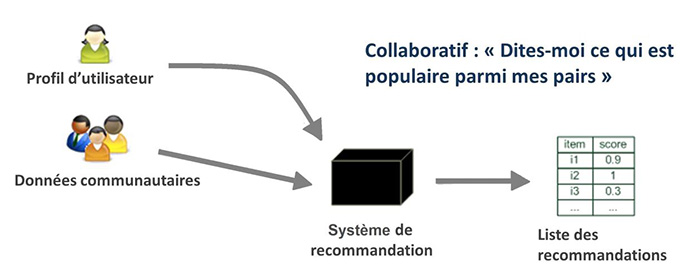
\includegraphics[width=95mm]{./src_img/rs-collaboratif}
  \caption{Un système de recommandation collaboratif\supercite{RSIntro}.}
  \label{fig:duo}
\end{figure}

\vspace{5mm}


Lorsqu'il y a des milliards de produits et un nombre conséquent de clients, il faut une énorme puissance de calcul pour calculer les recommandations. Il existe donc un problème sur l'évolutivité de ce système de recommandation. Lors de la première inscription d'un utilisateur, il est impossible de recommander des produits à cet utilisateur. Ce problème du démarrage a froid est contournable en demandant les préférences d'un utilisateur après son inscription. 

\vspace{5mm}

Aujourd'hui, Amazon a un algorithme de recommandation pour sa boutique. C'est un algorithme utilisant le filtrage collaboratif et plus spécifiquement "Item-To-Item". Lors de la lecture de la fiche "produit d'un article", Amazon suggère une liste d'autres produits en fonctions des clients ayant déjà acheté ce produit. Amazon personnalise aussi sa page d'accueil en fonction des achats précèdents ou des articles dans le panier du client. 

\vspace{5mm} 

\textit{« L’algorithme d’Amazon.com est basé sur le filtrage collaboratif appliqué aux éléments (Item-based collaborative filtering ou Item-to-Item). Le calcul en temps réel de cet algorithme s’adapte à la fois au nombre de clients et au nombre de produits dans le catalogue. L’algorithme construit une matrice de produits similaires en trouvant les produits que les clients ont tendance à acheter ensemble. »}\supercite{elsaNegre}

\vspace{5mm}

\begin{figure}[htp]
  \centering
  
\includegraphics[width=95mm]{./src_img/rs-collaboratif-sample}
  \caption{Amazon et la recommandationn collaborative.}
  \label{fig:duoB}
\end{figure}

\vspace{5mm}




\subsection{Le filtrage basé sur le contenu}

Pour les algorithmes de recommandation basés sur le contenu, le travail consiste à faire concorder les éléments du catalogue qui coïncident le mieux avec les préférences d'un utilisateur. Contrairement au filtrage collaboratif, ce type d'algorithme ne demande pas d'avoir un grand nombre d'utilisateur et peux s'appliquer à des structures plus petites. 

\vspace{5mm}


\begin{figure}[htp]
  \centering
  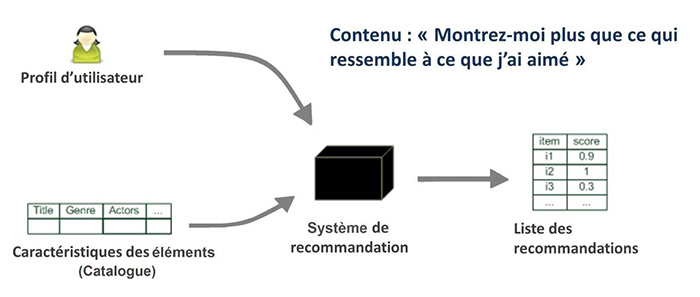
\includegraphics[width=95mm]{./src_img/rs-content}
  \caption{Un système de recommandation basé sur le contenu\supercite{RSIntro}.}
  \label{fig:trio}
\end{figure}

\vspace{5mm}


Premièrement, pour mettre en place ce type de recommandation, chaque éléments ou produits sont décrits par un nombre de caractéristiques connus et finis. Pour chaque utilisateur, il faut expirmer sous forme d'une liste ses intérêts et ses caractériques à nos produits ou nos éléments. 

\vspace{5mm}


La seconde étape pour la mise en place d'un algorithme de recommandation basé sur le contenu est de faire coïncider les caractéristiques des éléments et le profil de l’utilisateur. Ainsi, cela peut être mesuré de différentes manières :

\vspace{5mm}


\begin{itemize}
    \item \textbf{La mesure de similarité.}
    \vspace{2mm}
    \item \textbf{Le TF-IDF} (Term Frequency-Inverse Document Frequency) : consiste à déterminer un score de pertinence.  
    \vspace{2mm}
    \item \textit{«\textbf{Les techniques basées sur la similarité des espaces vectoriels} (les approches bayésiennes, les arbres de décision, etc.) couplées avec des techniques statistiques, lorsqu’il y a trop de mots-clés.»}\supercite{elsaNegre}

\end{itemize}

\vspace{5mm}



Les systèmes de recommandation basés sur le contenu présentent de nombreux avantages dont le démarrage à froid. Si un nouvel élément est ajouté au catalogue, il est simple de le recommander directement aux utilisateurs en fesant correspondre les caractéritiques et les centres d'intérêts d'un utilisateur. Avec ce système de recommandation, une personne avec des goûts atypiques différents de ceux de la base d'utilisateurs habituels n'est pas un problème. Pareil pour les éléments à recommander, un produit peu vendu ou atypique peu coïncider avec les goûts d'un nombre réduit d'utilisateur et donc être recommandé. 

\vspace{5mm} 

Malgrès les nombreux avantages que représente ce système de recommandation, il ne peut pas être appliquable à tous les utilisateurs. Les utilisateurs ayant consulté un grand nombre d’éléments posent un problème (une énorme masse d'information dans le profil de l’utilisateur à faire correspondre avec les propriétés des différents  éléments) et lorsqu’il n’existe pas d’historique (dans le cas d'un utilisateur qui commence à utiliser le système) par conséquence la recommandation pour ces deux cas peut-être difficile. Concernant les éléments à recommander, il est difficile de différencier deux éléments avec des caractéristiques similaires. Une étape difficile est la définition des caractéristiques de chaque utilisateur ainsi que la prise en compte de l'évolution des goûts et par conséquent des caractéritiques des utilisateurs.




\subsection{Le filtrage hybride}

Un système de recommandation hybride combine les approches collaboratives et basées sur le contenu. \textit{«Ce système de recommandation, peut utiliser à la fois  des connaissances extérieures et les caractéristiques des éléments, combinant ainsi des approches collaboratives et basées sur le contenu.»}\supercite{elsaNegre}


\vspace{5mm}

\begin{figure}[htp]
  \centering
  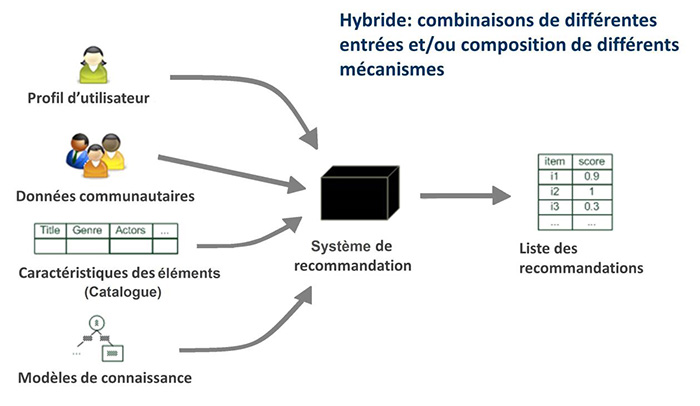
\includegraphics[width=95mm]{./src_img/rs-hybride}
  \caption{Un système de recommandation hybride\supercite{RSIntro}.}
  \label{fig:quatro}
\end{figure}

\vspace{5mm}

L'approche hybride est une combinaison de différentes approches, par conséquent sont but étant de présenter les avantages des approches qui la composent tout en limitant leurs inconvénients respectifs. Actuellement, il existe différentes catégories de combinaisons de systèmes de recommandation pour la création d'un système de recommandation hybride\supercite{RobinBurke,RSIntro}: 

\vspace{5mm}


\begin{itemize}
    \item \textbf{La combinaison monolithique} (monolithic hybridization design)\supercite{elsaNegre} : décrit une conception de l'approche hybride intégrant les aspects de différentes stratégies de recommandation en un seul algorithme.
    \vspace{2mm}
    \item \textbf{La combinaison parallèle} (parallelized hybridization design)\supercite{elsaNegre} : décrit une conception de l'approche hybride où sur la base de données d’entrée commune, les systèmes de recommandation fonctionnent de façon parallèles et indépendantes. Chacun produit une liste de recommandations distincte. Une étape ultérieure d’hybridation est nécessaire permettant de combiner le résultat en un ensemble final de recommandations.
    \vspace{2mm}
    \item \textbf{La combinaison tubulaire} (pipelined hybridization design)\supercite{elsaNegre} : décrit une conception de l'approche hybride où plusieurs systèmes de recommandation sont joints. Les données de sortie d’un système de recommandation devient une partie des données d’entrée du système de recommandation suivant.
    
\end{itemize}

\vspace{5mm}

\section{Le machine learning}

%http://penseeartificielle.fr/difference-intelligence-artificielle-machine-learning-deep-learning/#Le_machine_learning

\textit{«
Les systèmes de recommandation sont couramment utilisés en lien avec l’intelligence artificielle. Leurs capacités à fournir un aperçu global, à prédire les événements et à mettre en évidence des corrélations contribuent à expliquer leurs utilisations en IA. Par ailleurs, les techniques de Machine Learning sont fréquemment utilisées pour créer les algorithmes de recommandation. Par exemple, chez Arcbees, un système de prédiction des préférences de films a été construit, il utilise un réseau de neurones et les données de IMDb. Les réseaux de neurones peuvent effectuer rapidement des tâches complexes et manipuler facilement des données massives. En fournissant une liste de films comme entrées et en comparant la sortie avec la note de l’utilisateur, le réseau peut apprendre par lui-même la règle permettant de prédire les évaluations futures d’un utilisateur spécifique.»}\supercite{MachineLearn}

\section{L'approche de netflix}

%https://www.futura-sciences.com/tech/questions-reponses/informatique-netflix-fonctionne-algorithme-recommandations-8640/

%https://uxplanet.org/netflix-binging-on-the-algorithm-a3a74a6c1f59



Chez Netflix 80\%\supercite{p80} du contenu consommé par les utilisateurs est issu d'une recommandation. Fort de ce constat, le rôle du système de recommandation occupe une place centrale autant pour Netflix que pour ses utilisateurs. Ce système repose sur les utilisateurs, les caractéristiques des contenus et un algorithme. 

\vspace{5mm} 

Pour comprendre le besoins de ses utilisateurs, Netflix fait une analyse comportementale précise de chaque utilisateur. Ainsi, un contenu consommé sera utilisé pour recommander des series ou des films. Dans ce cas, Netflix utilise le machine learning pour dresser le portrait le plus précis possible de chaque utilisateur dont notamment : 


\vspace{5mm}


\begin{itemize}
    \item \textbf{La navigation précise}: combien de temps l'utilisateur met à trouver un contenu  et par quel moyen (strates, catégories,...).
    \vspace{2mm}
    \item \textbf{La temps de lecture d'un contenu }: permettant de déterminer si un contenu lancé est regardé en entier, à moitié ou partiellement  
    \vspace{2mm}
    \item \textbf{La notion de temps} : en fonction de la période de l'année, un type de contenu peut-être plus consommé par exemple les films de noël. Mais aussi en fonction de l'heure, par exemple en début de soirée peut-être que les utilisateurs consomment plus de films que de séries. 
    \vspace{2mm}
    \item \textbf{L'avis donné par l'utlisateur} : L'utilisateur peut donner son avis sur un contenu avec un icone "pouce vers le haut" ou "pouce vers le bas". 
\end{itemize}

\vspace{5mm}
%https://www.wired.co.uk/article/how-do-netflixs-algorithms-work-machine-learning-helps-to-predict-what-viewers-will-like

Une analyse du comportement seule ne permet pas de déterminer les séries et films à recommander à un utilisateur, il faut analyser le contenu et faire concorder le portrait de chaque utilisateur avec le contenu. L'ensemble du catalogue disponible sur Netflix est indexé pour décrire au mieux un centenu selon une immense bibliothèque de mots-clés. Le rôle de l'algorithme de machine learning est d'ordonnancer les données des utilisateurs et les contenus indexés. En pratique, le système de recommandation de Netflix appélé Cinematch analyse les scores cumulés de chaque contenu en utilisant une variante du coefficient de corrélation de Pearson avec tous les autres films afin de déterminer une liste de films « semblables » qui sont susceptibles de plaire à l'utilisateur. Puis, la partie en ligne et en temps réel du système calcule une régression multivariée\footnote{Le modèle de régression linéaire multiple est l’outil statistique le plus habituellement mis en œuvre pour l’étude de données multidimensionnelles. Cas
particulier de modèle linéaire, il constitue la généralisation naturelle de la régression simple.} basée sur ces corrélations pour déterminer une prédiction unique et personnalisée pour chaque film recommandable fondée sur ces scores.

%https://uxplanet.org/netflix-binging-on-the-algorithm-a3a74a6c1f59
%https://www.wired.co.uk/article/how-do-netflixs-algorithms-work-machine-learning-helps-to-predict-what-viewers-will-like
%https://mobilesyrup.com/2017/08/22/80-percent-netflix-shows-discovered-recommendation/